\documentclass[10pt,a4paper,UTF8]{ctexart}
\usepackage{geometry}%用于设置上下左右页边距
	\geometry{left=2.5cm,right=2.5cm,top=3.2cm,bottom=2.8cm}
\usepackage{xeCJK,amsmath,paralist,enumerate,booktabs,multirow,graphicx,subfig,setspace,listings,lastpage,hyperref}
\usepackage{amsthm, amssymb, bm, color, framed, graphicx, hyperref, mathrsfs}
\usepackage{mathrsfs}  
	\setlength{\parindent}{2em}
	\lstset{language=Matlab}%
\usepackage{fancyhdr}
\usepackage{graphicx}
\usepackage{listings}
\usepackage{xcolor}
\usepackage{float}

\definecolor{mKeyword}{RGB}{0,0,255}          % bule
\definecolor{mString}{RGB}{160,32,240}        % purple
\definecolor{mComment}{RGB}{34,139,34}        % green
\definecolor{mNumber}{RGB}{128,128,128} 

\lstdefinestyle {njulisting} {
	basewidth = 0.5 em,
	lineskip = 3 pt,
	basicstyle = \small\ttfamily,
	% keywordstyle = \bfseries,
	commentstyle = \itshape\color{gray}, 
	basicstyle=\small\ttfamily,
	keywordstyle={\color{mKeyword}},     % sets color for keywords
	stringstyle={\color{mString}},       % sets color for strings
	commentstyle={\color{mComment}},     % sets color for comments
	numberstyle=\tiny\color{mNumber},
	numbers = left,
	captionpos = t,
	breaklines = true,
	xleftmargin = 2 em,
	xrightmargin = 2 em,
	frame=tlrb,
	tabsize=4
}

\lstset{
style = njulisting, % 调用上述样式 
flexiblecolumns % 允许调整字符宽度
}

\pagestyle{fancy}
\lhead{\textsc{Foundation of Computing System}}
\rhead{\textsc{Nanjing University}}
\cfoot{\thepage}
\renewcommand{\headrulewidth}{0.4pt}
\renewcommand{\theenumi}{(\arabic{enumi})}


\definecolor{shadecolor}{RGB}{241, 241, 255}

\newcommand{\problemname}{待定义}
\newenvironment{problem}{\begin{shaded}\par\noindent\textbf{题目\  \problemname}}{\end{shaded}\par}
\newenvironment{solution}{\par\noindent\textbf{解答}\ }{\par}
\newenvironment{note}{\par\noindent\textbf{题目 \problemname 的注记}}{\par}

\begin{document}

\begin{center}
\LARGE\textbf{第十一章习题参考答案}
\end{center}

{\kaishu 包含题目:习题$11.8$、$11.10$、$11.12$、$11.14$、$11.16$和$11.17$}


% \begin{figure}[H]
% 	\centering
% 	\includegraphics[scale=0.3]{img/}
% \end{figure}

% \lstset{language=C}
% 	\begin{lstlisting}
	
% 	\end{lstlisting}



\renewcommand{\problemname}{11.8}
\begin{problem}
	对于如下程序
	\begin{enumerate}[(1)]
		\item 构建符号表
		\item 该程序实现了什么
	\end{enumerate}
\end{problem}

\begin{figure}[H]
	\centering
	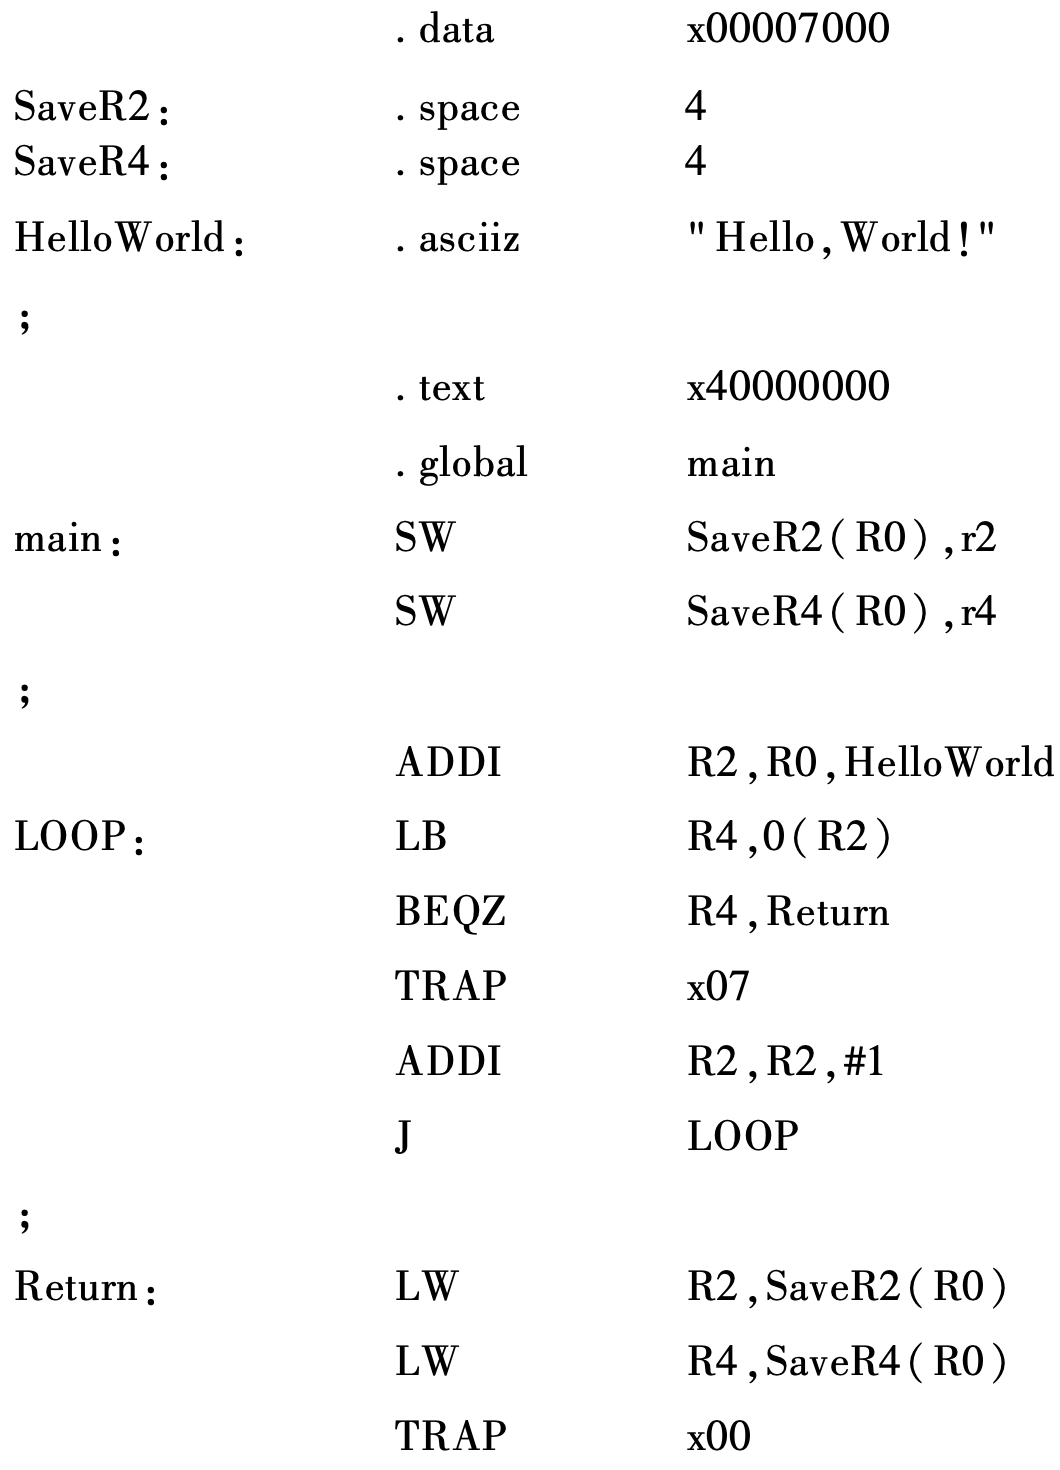
\includegraphics[scale=0.45]{img/11.8}
\end{figure}

\begin{solution}
	\begin{enumerate}[(1)]
		\item 构建符号表:
		\begin{table}[H]
			\centering
			\begin{tabular}{|l|l|}
			\hline
			符号         & 地址         \\ \hline
			SaveR2     & x0000 7000 \\ \hline
			SaveR4     & x0000 7004 \\ \hline
			HelloWorld & x0000 7008 \\ \hline
			main       & x4000 0000 \\ \hline
			LOOP       & x4000 000C \\ \hline
			Return     & x4000 0020 \\ \hline
			\end{tabular}
			\end{table}
		\item 该程序在不改变R2和R4值的情况下,输出“Hello, World!”。
	\end{enumerate}
\end{solution}


\renewcommand{\problemname}{11.10}
\begin{problem}
	对于如下程序
	\begin{enumerate}[(1)]
		\item 将该程序翻译为机器语言程序。
		\item 假设在这个程序执行之前,在NUM1中设置了一个正整数的值,该程序实现了什么?
	\end{enumerate}
\end{problem}

\begin{figure}[H]
	\centering
	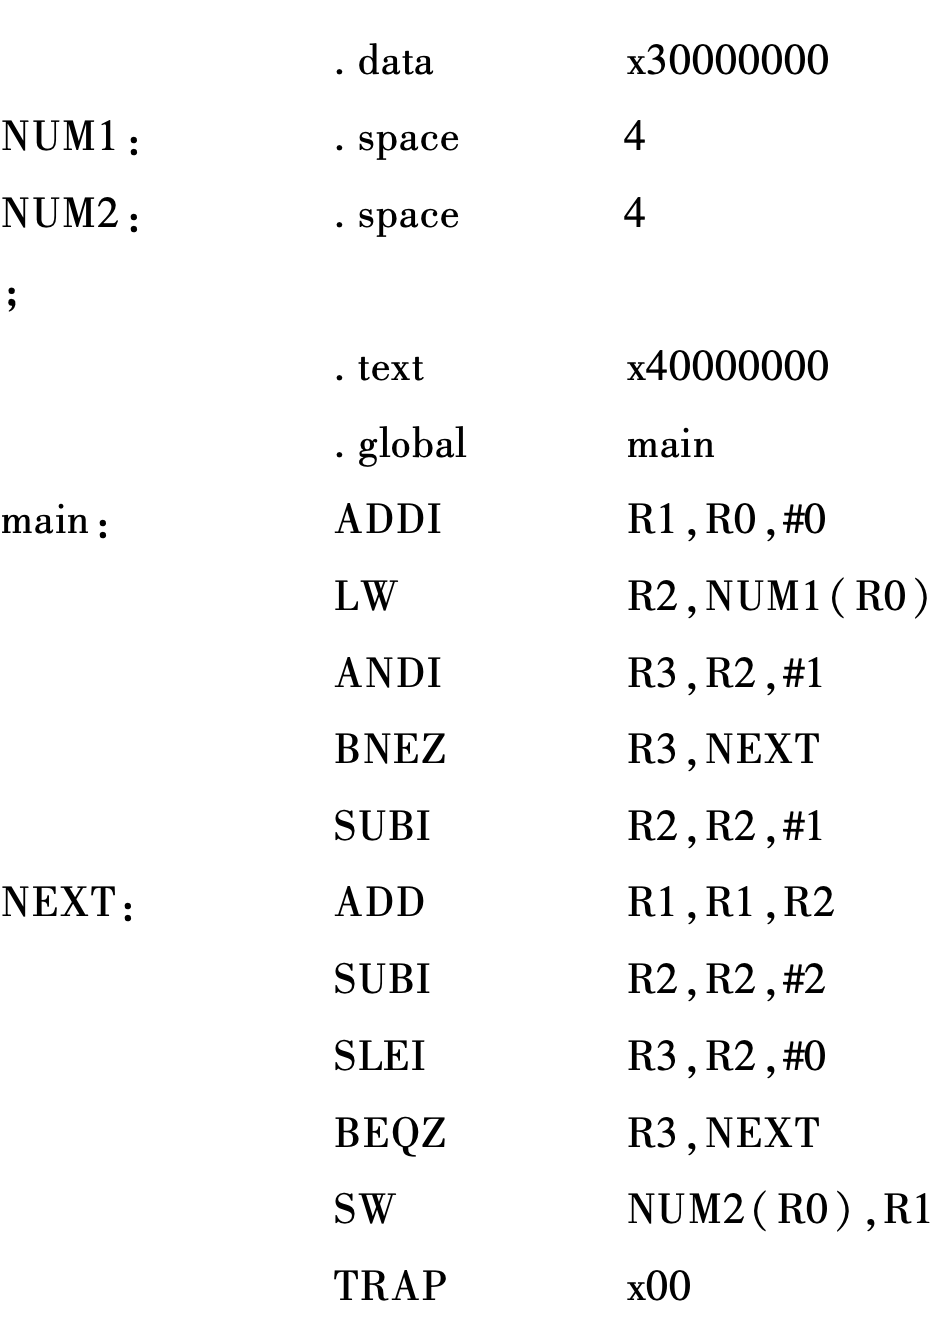
\includegraphics[scale=0.5]{img/11.10}
\end{figure}

\begin{solution}
	\begin{enumerate}[(1)]
		\item 第一步,建立符号表
		\begin{table}[H]
		\centering
			\begin{tabular}{|l|l|}
			\hline
			符号   & 地址         \\ \hline
			NUM1 & x3000 0000 \\ \hline
			NUM2 & x3000 0004 \\ \hline
			main & x4000 0000 \\ \hline
			NEXT & x4000 0014 \\ \hline
			\end{tabular}
			\end{table}
		
		第二步,翻译为机器语言
		\begin{table}[H]
		\centering
			\begin{tabular}{|l|l|l|}
			\hline
			地址         & 数据                                       & 解释               \\ \hline
			x4000 0000 & 000001 00000 00001 0000 0000 0000 0000 & \verb|ADDI  R1, R0, #0| \\ \hline
			x4000 0004 & 001100 00000 00100 0011 0000 0000 0000 & \verb|LHI  R4, x3000|    \\ \hline
			x4000 0008 & 011100 00100 00010 0000 0000 0000 0000 & \verb|LW  R2, x0000(R4)| \\ \hline
			x4000 000C & 001001 00010 00011 0000 0000 0000 0001 & \verb|ANDI  R3, R2, #1| \\ \hline
			x4000 0010 & 101001 00011 00000 0000 0000 0000 0100 & \verb|BNEZ  R3, NEXT|    \\ \hline
			x4000 0014 & 000011 00010 00010 0000 0000 0000 0001 & \verb|SUBI  R2, R2, #1| \\ \hline
			x4000 0018 & 000000 00001 00010 00001 00000 000001  & \verb|ADD  R1, R1, R2|   \\ \hline
			x4000 001C & 000011 00010 00010 0000 0000 0000 0010 & \verb|SUBI  R2, R2, #2| \\ \hline
			x4000 0020 & 010010 00010 00011 0000 0000 0000 0000 & \verb|SLEI  R3, R2, #0| \\ \hline
			x4000 0024 & 101000 00011 00000 1111 1111 1111 0000 & \verb|BEQZ  R3, NEXT|    \\ \hline
			x4000 0028 & 011101 00100 00001 0000 0000 0000 0100 & \verb|SW  x0004(R4), R1| \\ \hline
			x4000 002C & 110000 00000 00000 0000 0000 0000 0000 & \verb|TRAP  x00|         \\ \hline
			\end{tabular}
			\end{table}
		\item 该程序将不大于NUM1中的所有奇数求和,存入NUM2中。
	\end{enumerate}

\end{solution}


\renewcommand{\problemname}{11.12}
\begin{problem}
	如下程序存在一个错误,指出该错误并进行修复。该错误可以在汇编时还是在运行时被检测出来?
\end{problem}

\begin{figure}[H]
	\centering
	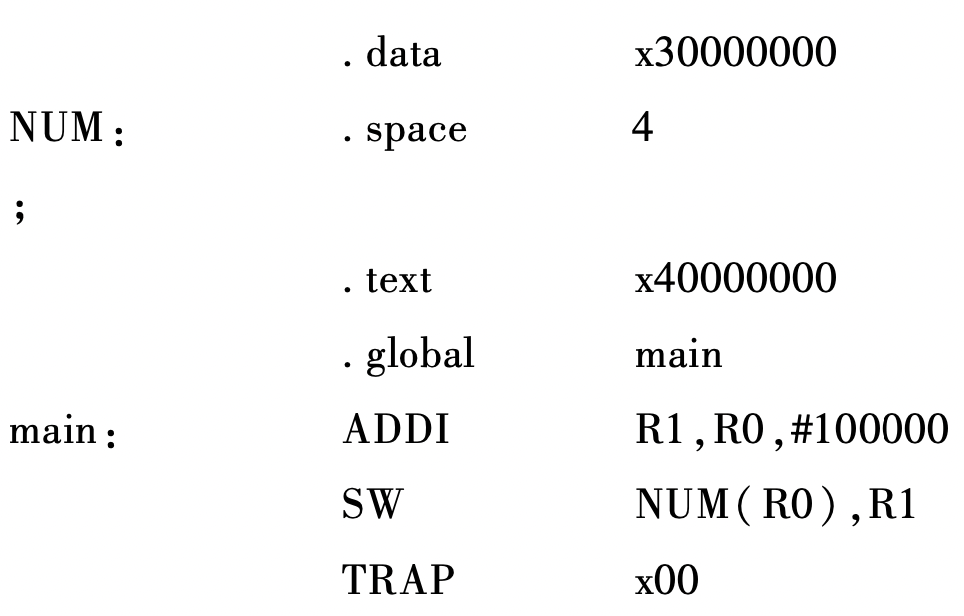
\includegraphics[scale=0.4]{img/11.12}
\end{figure}

\begin{solution}
	该程序的错误在 \verb|main: ADDI R1, R0, #100000| 中,I-型DLX指令中的立即数为16位补码整数,
	能表示的十进制范围为$-2^{15}\sim 2^{15}-1$,即$-32768\sim 32767$,100000在此范围之外。

	要修复该错误,可以将该指令替换为 \verb|LHI R2, x0001;  ADDI R1, R2, x86A0|	或
	\verb|ADDI R1, R0, #20000;|   \verb|ADDI R1, R0, #20000|


	由于汇编时立即数溢出,可知该错误是在汇编时被检测出来的。
\end{solution}


\renewcommand{\problemname}{11.14}
\begin{problem}
	如下DLX程序用于判断一个宇符串是否是“回文”(正向读和反向读都相同的宇符串),例如,strts
	就是回文。假设宇符串起始于存储单元x30000000。如果该字符串是回文,程序以R1的值为1结束,否则R1为
	0。填空,将程序补充完整。
\end{problem}

\begin{figure}[H]
	\centering
	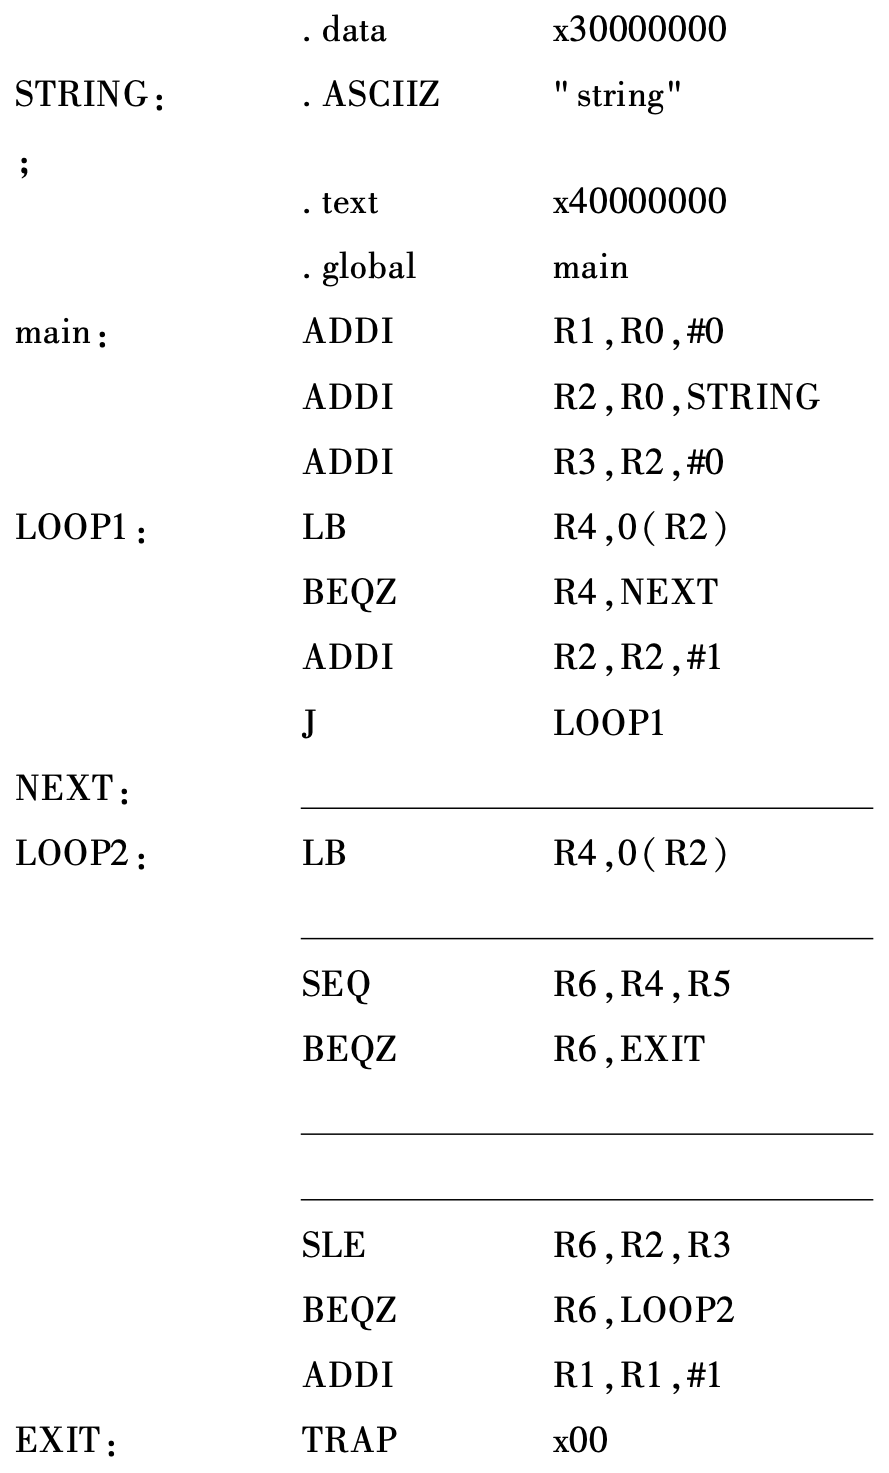
\includegraphics[scale=0.4]{img/11.14}
\end{figure}

\begin{solution}
	填入的代码依次为:
	\begin{lstlisting}
LB  R5, 0(R3)
ADDI  R2, R2, #1
ADDI  R3, R3, #1
ADDI  R1, R1, #1 或 ADDI  R1, R6, #0
	\end{lstlisting}

\end{solution}


\renewcommand{\problemname}{11.16}
\begin{problem}
	使用DLX的C编译器对如下局部变量声明进行编译,写出DLX汇编代码。
	\begin{lstlisting}[language=C]
char c = 'c';
int x = 5;
int y;
	\end{lstlisting}
\end{problem}

\begin{solution}
	\begin{lstlisting}
ADDI  R5, R0, x63 或 ADDI  R5, R0, #99
SW  -4(R30), R5
ADDI  R5, R0, #5
SW  -8(R30), R5
ADDI  R5, R0, #0
SW  -12(R30), R5
	\end{lstlisting}
\end{solution}


\renewcommand{\problemname}{11.17}
\begin{problem}
	使用DLX的C编译器对如下 \verb|switch| 语句进行编译,写出DLX汇编代码。
	\begin{lstlisting}[language=C]
int i, j, k, x;
...
switch (i){
	case 0:
		x = k + j;
   		break;
	case 1:
    	x = k - j;
    	break;
  	case 2:
    	x = i + k;
    	break;
  default:
    	x = i - k;
}
	\end{lstlisting}
\end{problem}

\begin{solution}
	\begin{lstlisting}
				ADDI R16, R0, #0; i
				ADDI R17, R0, #0; j
				ADDI R18, R0, #0; k
				ADDI R19, R0, #0; x
				……
				SEQI R1, R16, #0
				BNEZ R1, Case_0
				SEQI R1, R16, #1
				BNEZ R1, Case_1
				SEQI R1, R16, #2
				BNEZ R1, Case_2
				J Case_default
Case_0:			ADD R19, R18, R17
				J Done
Case_1:			SUB R19, R18, R17
				J Done
Case_2:			ADD R19, R16, R18
				J Done
Case_default:	SUB R19, R16, R18
				J Done
Done:			……
	\end{lstlisting}
\end{solution}


\end{document}
